\documentclass[12pt]{article}
%\usepackage{amsmath}
\usepackage{graphicx}
\usepackage{wrapfig}
\usepackage[export]{adjustbox}
\usepackage{enumitem}
\usepackage{subfigure}%
%\usepackage{enumerate}
\usepackage{natbib} %comment out if you do not have the package
\usepackage{url} % not crucial - just used below for the URL 
\usepackage{caption}
\usepackage{subcaption}
%\pdfminorversion=4
% NOTE: To produce blinded version, replace "0" with "1" below.
\newcommand{\blind}{0}

% DON'T change margins - should be 1 inch all around.
\addtolength{\oddsidemargin}{-.5in}%
\addtolength{\evensidemargin}{-1in}%
\addtolength{\textwidth}{1in}%
\addtolength{\textheight}{1.7in}%
\addtolength{\topmargin}{-1in}%


\begin{document}

%\bibliographystyle{natbib}

\def\spacingset#1{\renewcommand{\baselinestretch}%
{#1}\small\normalsize} \spacingset{1}


%%%%%%%%%%%%%%%%%%%%%%%%%%%%%%%%%%%%%%%%%%%%%%%%%%%%%%%%%%%%%%%%%%%%%%%%%%%%%%

\if0\blind
{
  \title{\bf Neural network-based fall detector}
  \author{Frenki Shqepa\hspace{.2cm}\\
    Università degli Studi di Brescia\\
    }
     \date{}
  \maketitle
  \thispagestyle{empty}
} \fi

\if1\blind
{
  \bigskip
  \bigskip
  \bigskip
  \begin{center}
    {\LARGE\bf Title}
\end{center}
  \medskip
} \fi

\bigskip
\bigskip
\bigskip
\bigskip
\bigskip
\bigskip
\bigskip
\bigskip
\bigskip
\bigskip
\bigskip

\subsection*{\centering Abstract}
This report describes the path our group followed to develop a wearable fall detection device based on an artificial intelligence algorithm.
We start with the description of the problem, then move on to the preprocessing and feature extraction operations, followed by the classifier and the results obtained. More attention is given to the data processing steps.

\clearpage
\pagenumbering{arabic} 



\newpage
\spacingset{1.5} % DON'T change the spacing!

\section*{\centering Introduction}

\label{sec:intro}

\subsection*{Why do you need a fall detector?}
Falls are the second leading cause of death from unintentional injuries worldwide, and each year an estimated 684,000 people die from them globally.
Another problem concerns rescue: in fact, it can take hours before a person, perhaps fallen in a place without someone nearby, is rescued[1].
If a person is alone, it is difficult to prevent the fall, but it is possible to act on post-trauma rescue. With this purpose, a wearable device has been developed that can detect a fall and automatically send a message to a selected person, asking for help.


\subsection*{How can a fall be detected?}
You want to monitor the movement of a person, so the most suitable sensors are inertial sensors, namely \textbf{accelerometer} and \textbf{giroscope}. A very simple approach to detect a fall is to define a threshold, which when exceeded, results in the detection of the event. One must take into account the inter- and intra-variability of a fall, so a simple threshold may not be fit for purpose, because a person may fall the same way on two different occasions, but the signals collected are different (Figure 1).

\begin{figure}[!h]
    \centering
    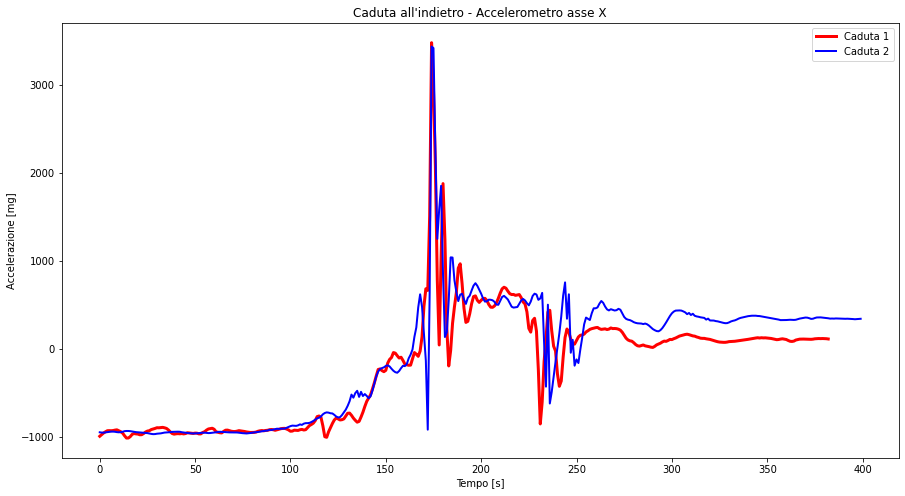
\includegraphics[width=5in]{confrontointerintra.png}
    \caption{Signals acquired from Accelerometer, X-axis, for two backward falls.}
    \label{fig:label}
\end{figure}

\subsection*{Development Roadmap}
The development process involves the acquisition of useful signals. These data come from the SensorTile.Box, a development kit distributed by STMicroelectronics. The Inertial Measurement Unit (IMU) - LSM6DOX - was used, which includes an accelerometer and a gyroscope, for a total of \textbf{six degrees of freedom} (three axes for each sensor).

\begin{wrapfigure}{r}{0.60\textwidth}
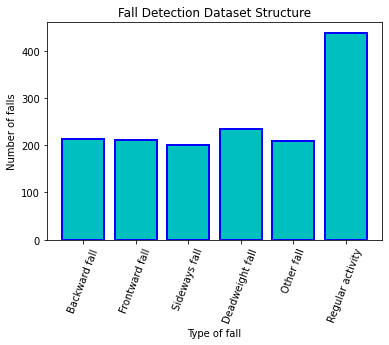
\includegraphics[width=0.9\linewidth]{dataset_structure.png} 
\caption{Structure of the dataset used.}
\label{fig:wrapfig}
\end{wrapfigure}

The data was acquired via USB with the software \emph{SensiML Data Capture Lab}, allowing to build the dataset.
When talking about artificial intelligence, it is indeed very important to have a large and varied dataset. For the goals set, 1503 signals were collected, distributed as in Figure 2.

The next step is the \textbf{extraction of features}, fundamental for a good training of the classifier.
Then we can proceed with the development of the \textbf{neural network}, the classifier that allows to detect a fall.
The last step is the deployment of the model on the SensorTile.Box and use with the connected app. A schematic of the development path can be seen in Figure 3.


\begin{figure}[!h]
    \centering
    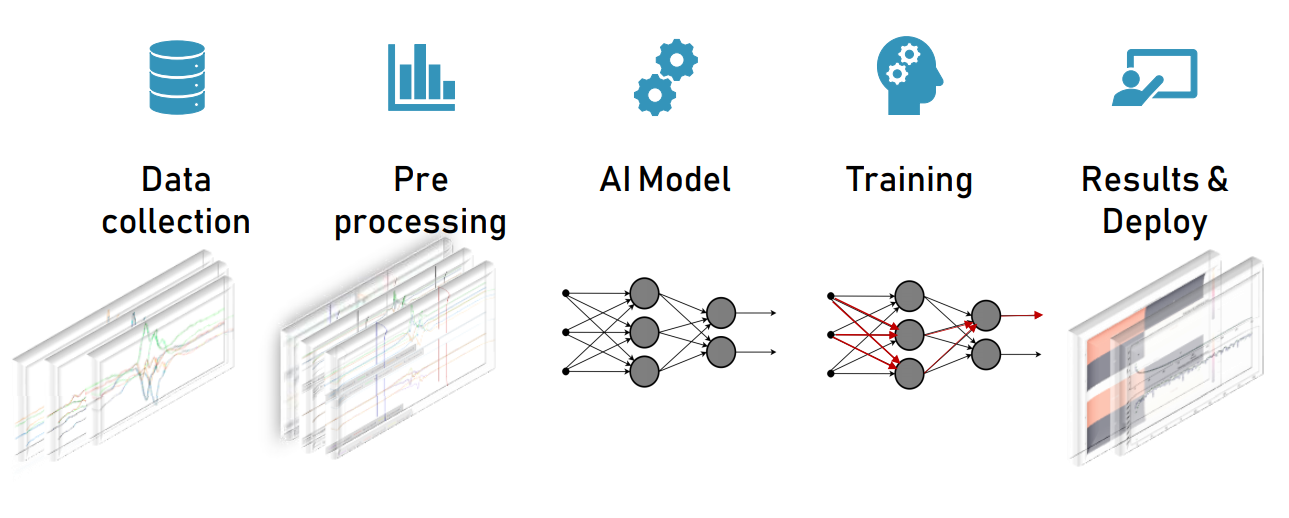
\includegraphics[width=4.97in]{roadmap.PNG}
    \caption{Development Pathway.}
    \label{fig:label}
\end{figure}

\section*{\centering Tools and Methods}
\label{sec:m&s}

\subsection*{Tools used}
Considering Figure 1, we see that there are very sharp peaks in the signals, which are certainly important when analyzing for feature extraction. A fundamental step is the choice of \textbf{sampling frequency}, so as not to lose important data. Choosing a very high one may be fine, but remember:
\setlist{nolistsep}
    \begin{itemize}[noitemsep]
        \item The device does not need to reconstruct the initial signal (so compliance with Shannon's Theorem is not essential);
        \item The size in terms of bytes of the acquired signal may increase due to the increased number of samples.
    \end{itemize}
The problem concerns low sampling frequencies. If a frequency of, for example, 3 Hz is used, important data, such as peaks, will certainly be lost. Please note that Sensiml Data Capture Lab was used, which allows the use of a different number of sampling frequencies, but also the application ST BLE Sensor, with the function of signal acquisition via Bluetooth Low Energy. The latter application also makes multiple sampling frequencies available, so by "cross-referencing" the available frequencies, a sampling frequency of 104 Hz was chosen.
We have to make some considerations also on the measuring range of the accelerometer: is it suitable to detect a fall? Exclude falls in which sensitive organs or body parts (e.g. temples, neck) are hit. A human being can withstand accelerations from 4g to 6g, up to 9g for a few seconds (do not consider trained persons). The accelerometer has a measuring range of (-4 ÷ +4)g, therefore suitable for the purpose. As for the gyroscope, the measuring range is (-2000 ÷ +2000)dps, which, in the full-scale value, corresponds to a high number of complete revolutions, to be excluded in the case of a normal fall.
It is concluded that the two sensors have suitable measuring ranges. It is then the data from these two sensors that are processed and fed into the classifier. Among the downsides of inertial sensors is the absence of a reference system, so the dataset was created by falling on a mattress, with the microcontroller in the pocket, varying the orientation as much as possible. In this way, the neural network is able to make a prediction regardless of the pocket the device is in and its orientation.
\subsection*{Why a neural network?}
\begin{wrapfigure}{r}{0.45\textwidth}
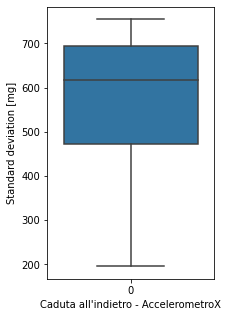
\includegraphics[width=0.8\linewidth]{boxplot_std.png} 
\caption{Boxplot of standard deviations in a group of 22 backward falls, relative to the x-axis of the accelerometer.}
\label{fig:wrapfig}
\end{wrapfigure}
Consider again the use of a threshold, placed for example on the standard deviation of the data from the x-axis accelerometer. 

As seen in Figure 4, the standard deviation varies even among falls of the same type, so it is difficult to rely solely on a threshold to determine a fall.
The considerations just made led to discard the use of a threshold and deviate to the use of a neural network. Artificial intelligence was chosen because it allows to detect a fall thanks to the analysis of multiple features, not just one property of the signal, but also because it allows to find non-linear relationships between inputs, difficult to highlight with other algorithms.

\subsection*{Preprocessing}

Before extracting features, it is necessary to process the data in order to optimize the extraction of important features as much as possible.
First, we apply a \textbf{finestration} to each signal. 
The main goal of this operation is to increase the size of the dataset (Figure 5), so that each window is treated as if it were a separate signal.
\begin{wrapfigure}{l}{0.40\textwidth}
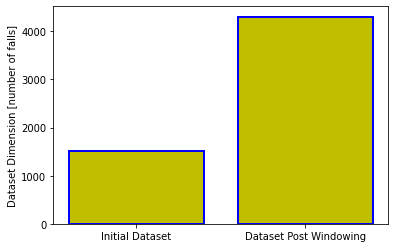
\includegraphics[width=0.7\linewidth]{dataset_dimension.png} 
\caption{Size of the dataset before and after fenestration.}
\label{fig:wrapfig}
\end{wrapfigure}
Windowing consists in dividing each signal into windows of a given size, with the possibility of overlapping between them. To choose these two parameters, it is necessary to analyze the dynamics of a drop. A fall lasts between 2 and 4 seconds, however the phase in which the ascent that leads to the peak of the acquired signal begins, to which we then add the impact, can be framed in a window of about a second and a half.

We therefore decided to use a window of 1.5s, corresponding, given a sampling rate of 104Hz, to 156 samples. We found the first parameter. 
As for the overlapping region between windows, it was decided to size it so that only the peak would fit inside. In this way, if a window can not include the entire peak, the next window, thanks to an overlap of 52 samples (value determined experimentally), will contain it all. Graphical representation of the windowing in figure 6.
To recap:
\begin{itemize}
  \item Window size equal to 156 samples, which contains the most useful portion of the fall;
  \item Overlap window size equal to 52 samples, such that at least one of two adjacent windows, contains the peak relative to the fall.
  \end{itemize}
Despite the application of fenestration, the size of the dataset is still too small for the creation of a multiclass classifier, so it was considered to work on a binary classifier (fall - not fall).
\begin{figure}[!h]
    \centering
    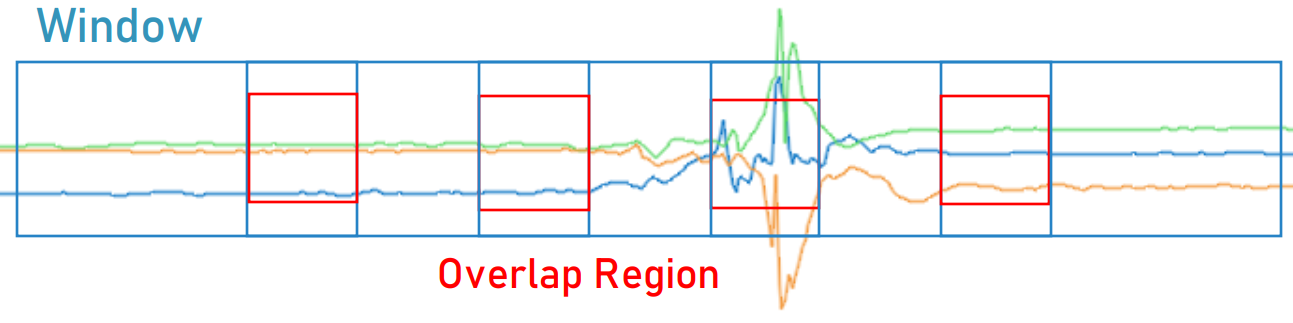
\includegraphics[width=4.97in]{overlap.PNG}
    \caption{Windowing Operation.}
    \label{fig:label}
\end{figure}

\subsection*{Featrures extraction}
This is a critical step, as mentioned several times. 
At first glance, you can think of using as many features as possible, the rest is done by the neural network. You have to consider that the network must work on a microcontroller, in real-time and the power consumption must be minimized. These are details that are also addressed at the end of the development, when you have data available to make comparisons and modifications, but you have to start the feature extraction process with these concepts already in mind.
One possible approach for this is to extract a group of features and then use a feature selector. This algorithm allows you to give a degree of importance to each feature applied to the data in the dataset. In this way you have the "ranking" of the most important properties and you can then select which ones to eliminate, in order to reduce the size of the input data to the network. Alternatively you can define the number of features you want and the selector will automatically delete them.


Consider any signal in figure 1. It is evident that the signal is not periodic, so you can exclude periodic features, such as period. 
The falls do not have the same duration and the first peak is not always at the same time from the beginning of the fall, so we can exclude these types of temporal features.
\begin{wrapfigure}{l}{0pt}
  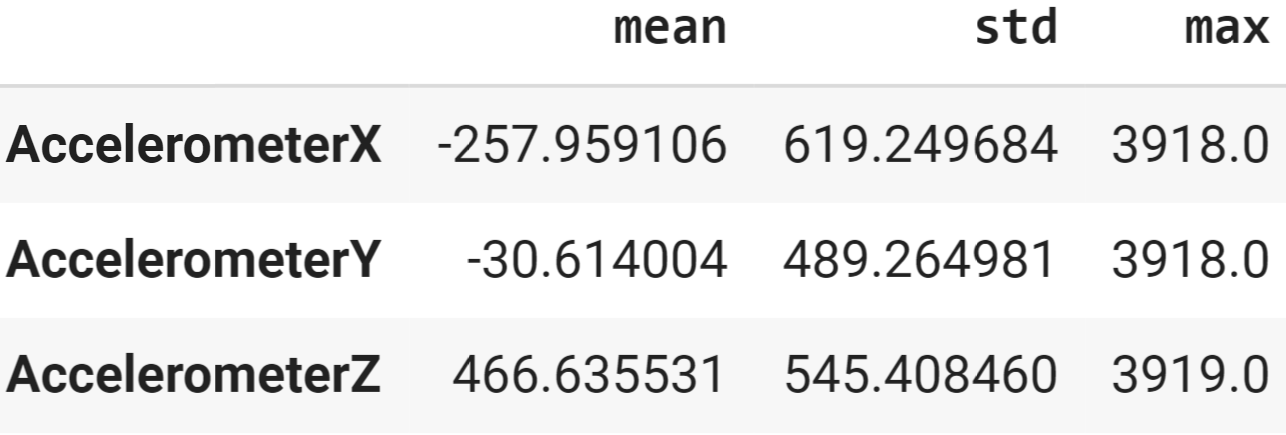
\includegraphics[scale=0.2]{std.PNG}
  \caption{Parameters compared on the group of twenty-two backward falls.}
\end{wrapfigure}
Looking at the signals, one notices that there is a lot of variation on the vertical axis, all the way up to very high peaks. If we analyze figure 7, the standard deviation has high values, not much smaller than the peak values ('max' in figure 7), so this is definitely a feature to consider.
An important property of signals is energy, so we can extract energy features, such as average and total energy. 
The falls belonging to the same class, considering the due inter- and intra-individual differences, have similar waveforms, then the add features belonging to this group, such as the 'Global Peak to Peak', which calculates the distance between the two largest peaks in modulus. 
Frequency features can also be analyzed, such as 'Dominant Frequency', which calculates the dominant frequency for each specified signal. For each column, this feature finds the frequency at which the signal has the maximum power.

After choosing features, you can move on to using the Forest Feature Selector. Random forests consist of hundreds of trees, but not everyone sees all features or all observations, this ensures that the trees are de-correlated and therefore less prone to over-fitting. Each tree is also assigned a sequence of yes/no questions based on a single or combination of features (e.g. std<value). At each node (i.e., at each question), the trees divide the dataset into 2 groups, each hosting observations that are more similar to each other and different from those in the other group. Therefore, the importance of each feature is derived from how "pure" each of the groups is.

For the feature extraction process, we relied on functions from the SensiMl Python library.

\begin{wrapfigure}{r}{0pt}
  \includegraphics[scale=0.5]{pipeline.PNG}
  \caption{Main steps of the preprocessing phase.}
\end{wrapfigure}
The last operation to perform before training the network, is the scaling of the features. Often the values of some features are orders of magnitude higher than those of other properties and many times they are in different ranges of values, even very different. 
The scaling is then carried out in a range of values (0-1, 0-255), in order to bring the values in the same intervals, thus making fair the contributions of each feature in the network, but also to reduce the calculation time (not to be neglected).
The summary of the preprocessing phase can be seen in Figure 8, where "generatorset" includes feature extraction and the forest selector.

\subsection*{The classifier - the neural network}
To conclude the process, a decision rule is needed to distinguish a fall from a regular activity.
After working on the features, we move on to the creation of the neural network. Two architectures were analyzed, Artificial Neural Network and Recurrent Neural Network. It must be remembered that the network must work on a microcontroller, which has a limited memory (2MB FLASH in the SensorTile.Box), which also can not be dedicated only to the decision-making algorithm. Two comparisons were made between the architectures, in terms of size in bytes and accuracy, both evaluated as the number of features used to train the network increases (figure 9).
From the graph on the left in figure 9 it is evident the similar-exponential increase of the model based on LSTM layers, while the artificial neural network maintains a reduced size, even for a high number of features. Looking at the graph on the right, we see that after about 10 features, the accuracy is not very different in the two architectures, so for the same latter metric, the difference is made by the model size.
The final choice was influenced by the fact that the framework used to develop the neural network, Tensorflow, does not currently support conversion of LSTM layers to binary code, leading to the choice of the artificial neural network, trained with 42 features.
\begin{figure}[!h]
    \centering
    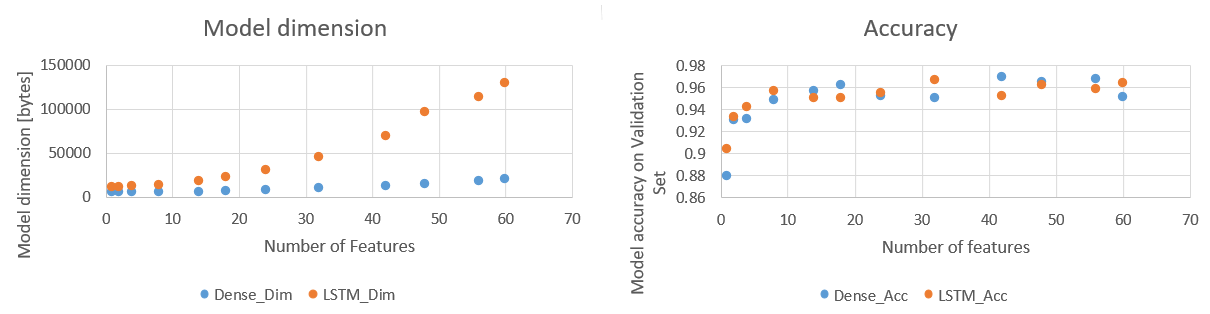
\includegraphics[scale=0.5]{metrics.png}
    \caption{Metrics of the two models compared as the number of features used to train the network increased.}
    \label{fig:label}
\end{figure}

\section*{\centering Results}
\begin{wrapfigure}{l}{0pt}
  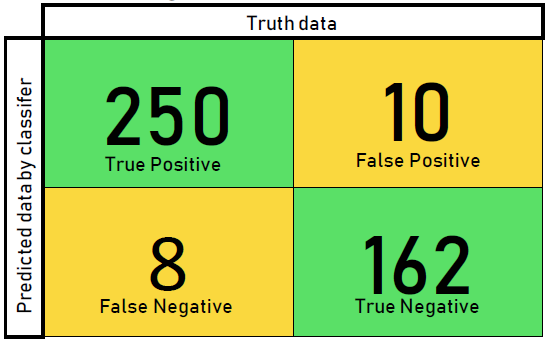
\includegraphics[scale=0.5]{conf_mat}
  \caption{Classifier confusion matrix.}
\end{wrapfigure}
To evaluate the goodness of fit of a classifier, the most commonly used method is the confusion matrix (Figure 10), which compares actual data and model predictions. In the present case, we want to reduce the false negative rate as much as possible, i.e., when a person falls, but the classifier does not detect the fall. This is in fact the biggest problem, as it does not allow the connected application to send a help message, thus rendering the device useless.
From the confusion matrix we can derive some basic parameters:

\begin{equation}
 {True Positive Rate_\%} = \frac{True Positive}{True Positive + False Negative} = 96.90\%
\end{equation}

\begin{equation}
{True Negative Rate_\%} = \frac{True Negative}{True Negative + False Positive} = 94.19\%
\end{equation}
   
\begin{equation}
 {False Negative Rate_\%} = \frac{False Negative}{True Positive + False Negative} = 3.10\%
\end{equation}

\begin{equation}
{False Positive Rate_\%} = \frac{False Positive}{True Negative + False Positive} = 5.81\%
\end{equation}    

\begin{equation}
{Accuracy_\%} = \frac{True Positive + True Negative}{Negative + Positive} = 95.81\%
\end{equation}

\begin{wrapfigure}{l}{0pt}
  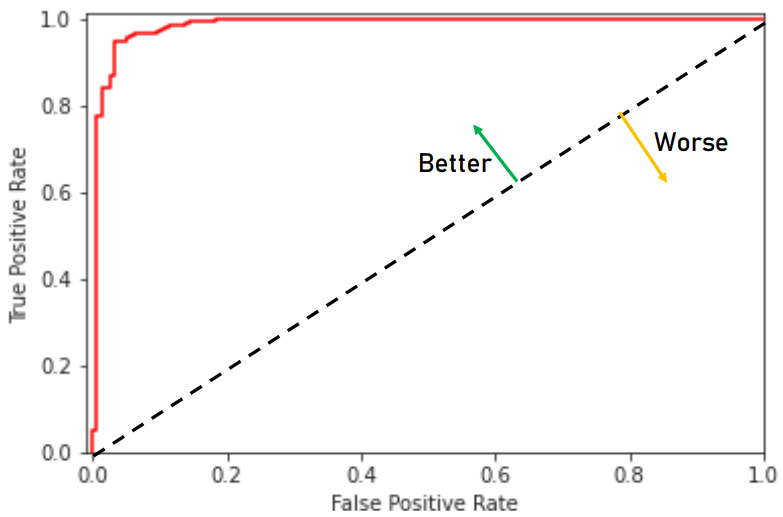
\includegraphics[scale=0.35]{roc.PNG}
  \caption{Curva ROC.}
\end{wrapfigure}





Another method of assessing the goodness of the model is the ROC (Receiver Operating Characteristic) curve. 
This is a probability curve, from which the AUC (Area Under Curve) can be derived, which instead represents the degree or measure of separability. 
The AUC tells how well the model is able to distinguish between classes. The classifier used has an AUC = 0.98, close to 1, which is the maximum value, only possible in an ideal classifier (Figure 11).

\section*{\centering Next steps}.
It has been established that the binary classifier works well, has high accuracy and very low false negative rate.
However, the goal is to create a multiclass classifier, so the first step is to collect new data to increase the size of the dataset.
You can also think of breaking away from using the SensorTile.Box, as there are many unnecessary sensors for our device, which only increase the price of the microcontroller. The desire is to design a microcontroller from scratch, suitable for our problem.
We also want to develop our own library, so as not to depend on too expensive softwares, but also to avoid the creation of code in the cloud that, as much as it may be convenient, introduces problems related to the security of data acquired, especially if personal.

\section*{\centering Sitography}
[1] World Health Organization, \emph{Falls}, 2021. URL: https://www.who.int/news-room/fact-sheets/detail/falls.










\end{document}
